\begin{task}{1, Setting up the Vadere environment}
In this task, we will explore the Vadere software, a valuable tool for simulating pedestrian movement. The objective is to use its graphical interface to recreate specific scenarios: RiMEA scenarios 1 (straight line) and RiMEA scenarios 6 (corner), along with the "chicken test" from the first exercise. Employing the Optimal Steps Model (OSM) with its standard template, our aim is to observe and analyze model trajectories, visualizations, user interface interactions, and test results. Additionally, we will compare these outcomes with the cellular automaton developed in the first exercise to identify any similarities and differences. This exploration allows us to better understand Vadere's capabilities in simulating pedestrian movement. \textit{Note that for task 1,2,3 the vadere project with its scenarios are placed in the folder} \verb+Exercise-2\vadere-project-task123+

\paragraph{RiMEA scenario 1}
In this scenario, the goal is to demonstrate that an individual in a 2 m wide and 40 m long corridor, with a predefined walking speed, will cover the distance within the corresponding time period.

To simulate this scenario in Vadere, as can be seen in Figure \ref{rimea1_setup}, the \texttt{Obstacle} tool was utilized to create two gray rectangles of size $1 \times 42$ in the center of a $50 \times 50$ map, representing the corridor. The rectangles are spaced 2 units apart. Additionally, the \texttt{Target} tool was employed to create an $2 \times 1$ orange rectangle on the right side to represent the exit. On the left side, the \texttt{Pedestrian} tool was used to introduce an individual with a walking speed of $1.33 \, \text{m/s}$, represented by a blue color.

\begin{figure}[H] 
\centering
\subfigure[RiMEA 1 setup\label{rimea1_setup}]{
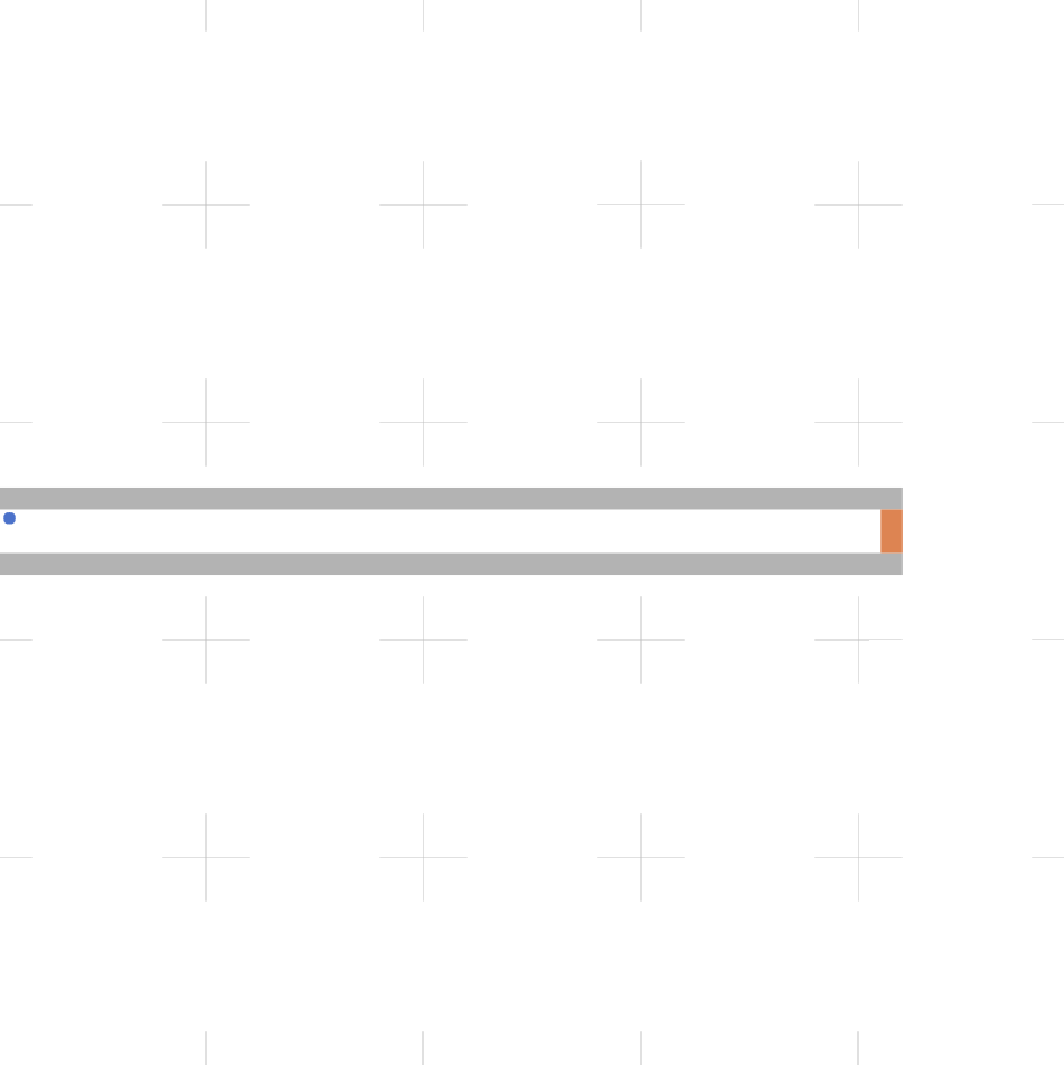
\includegraphics[scale=0.35]{report-template/images/rimea-1-setup.png}}
\subfigure[RiMEA 1 finshed]{
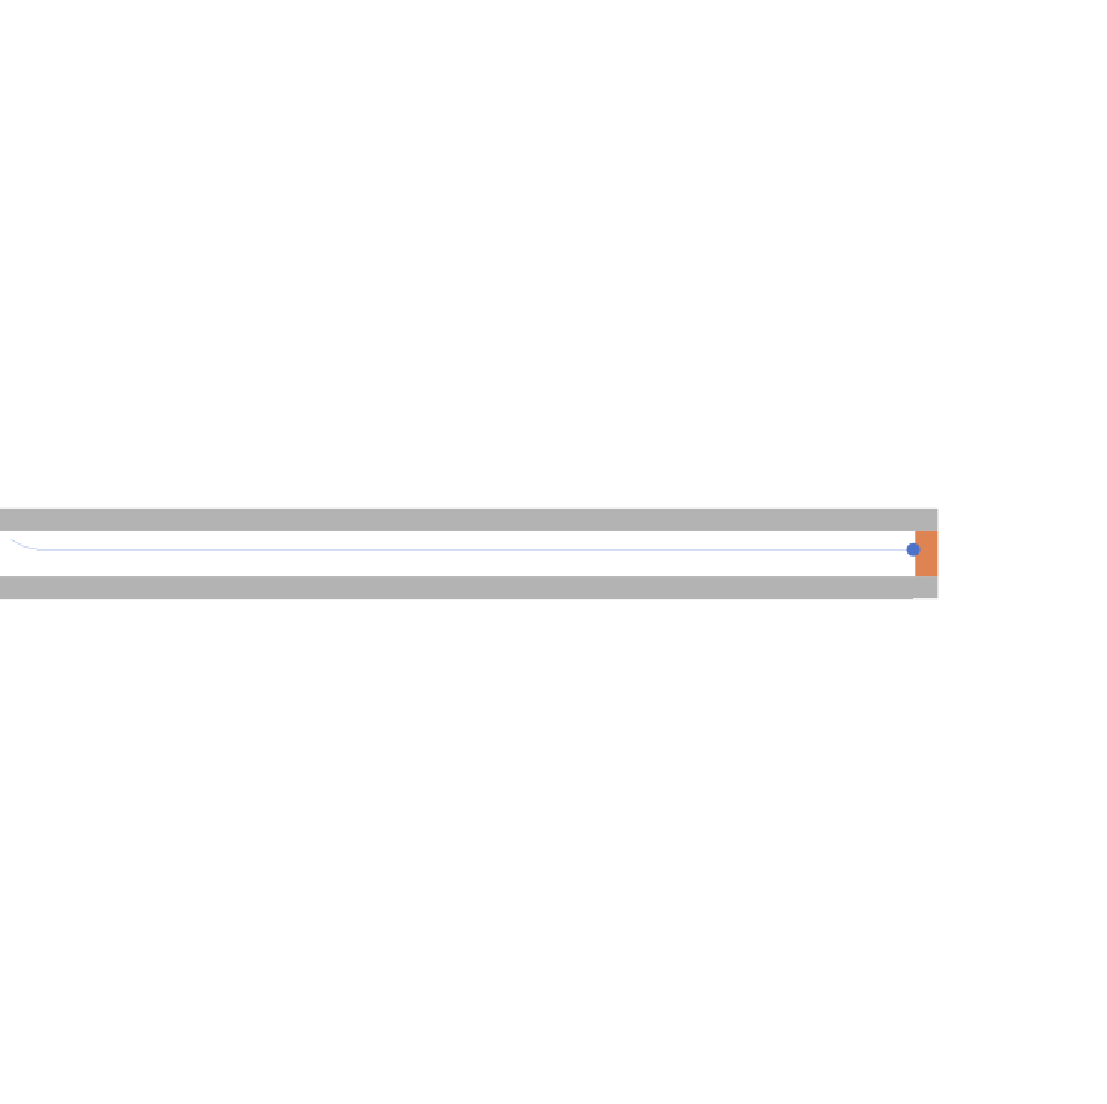
\includegraphics[scale=0.35]{report-template/images/rimea-1-fin.png}}
\subfigure[ex1 RiMEA 1 setup]{
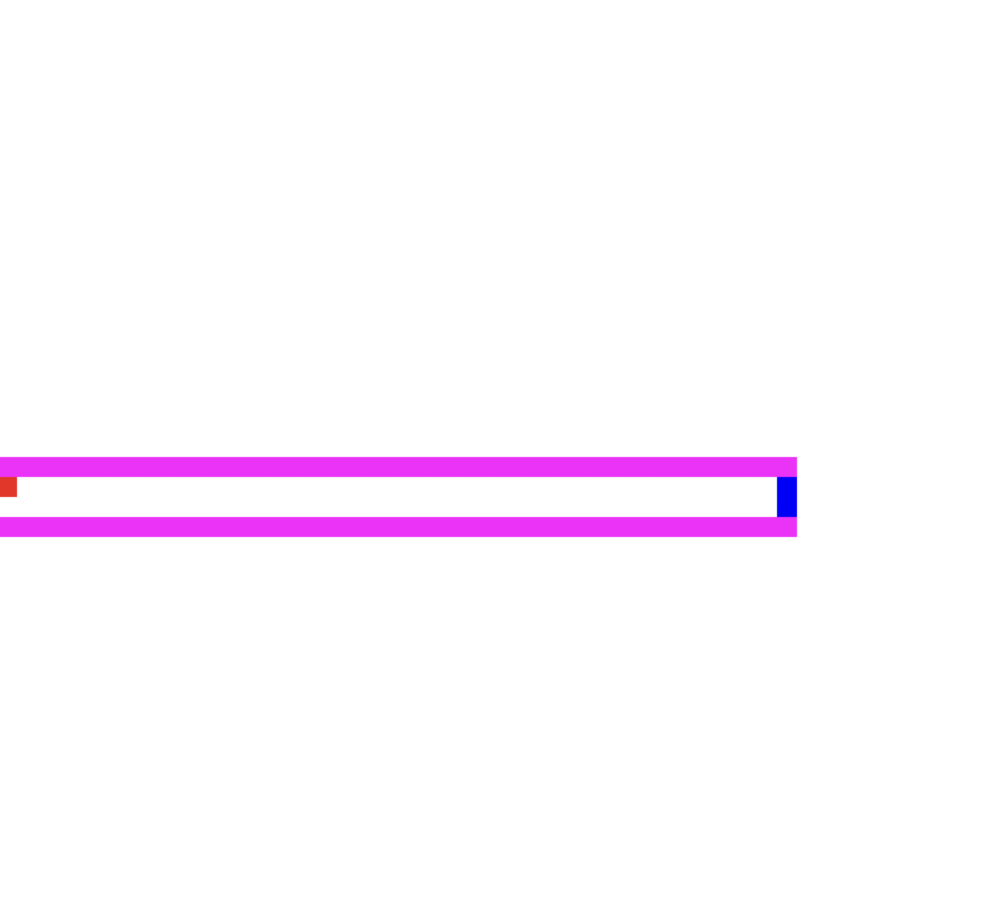
\includegraphics[scale=0.35]{report-template/images/old-rimea-1-setup.png}}
\subfigure[ex1 RiMEA 1 finshed]{
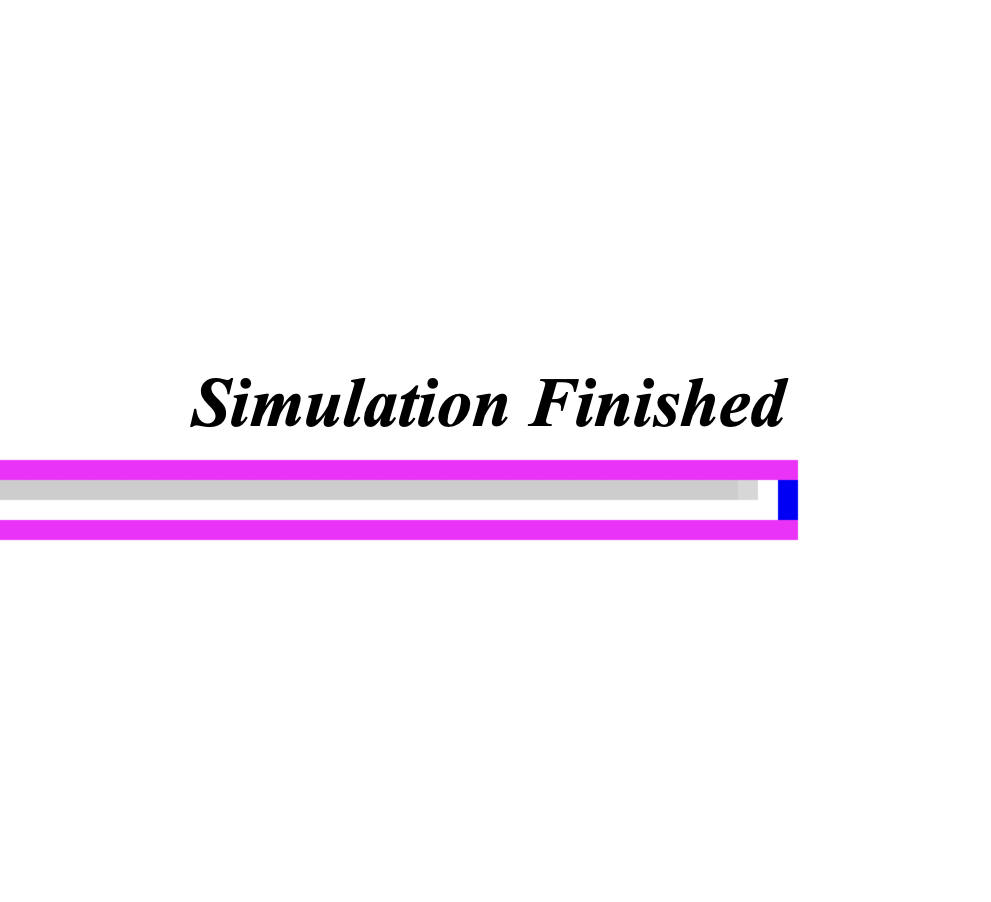
\includegraphics[scale=0.35]{report-template/images/old-rimea-1-fin.png}}
\caption{Comparison of RiMEA 1 simulations}
\label{rimea1}
\end{figure}

\newpage
The Figure \ref{rimea1} illustrates a comparison between RiMEA Scenario 1 in exercise 1 and this simulation. Similarities can be observed, as pedestrians take approximately the same amount of time to traverse the entire path. However, a notable distinction lies in the paths traversed by pedestrians in each experiment. In the simulation in exercise 1, the pedestrian moves in a straight line throughout the journey. However, in the this simulation with the OSM, the pedestrian moves toward the midpoint of the corridor during the forward movement, and then walks in a straight line to complete the route.

\paragraph{RiMEA scenario 6}
The purpose of this scenario is to demonstrate that a group of twenty individuals, moving towards a corner that turns left, will successfully navigate around it without passing through walls.

\begin{figure}[H] 
\centering
\subfigure[RiMEA 6 setup\label{rimea6_setup}]{
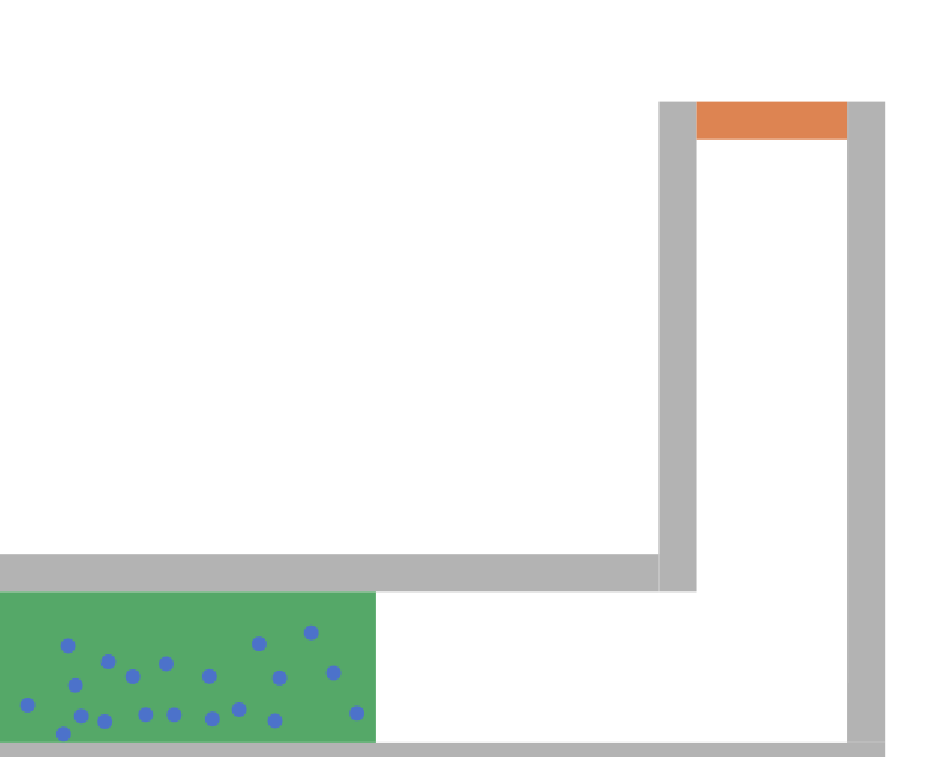
\includegraphics[scale=0.25]{report-template/images/rimea-6-setup.png}}
\subfigure[RiMEA 6 run]{
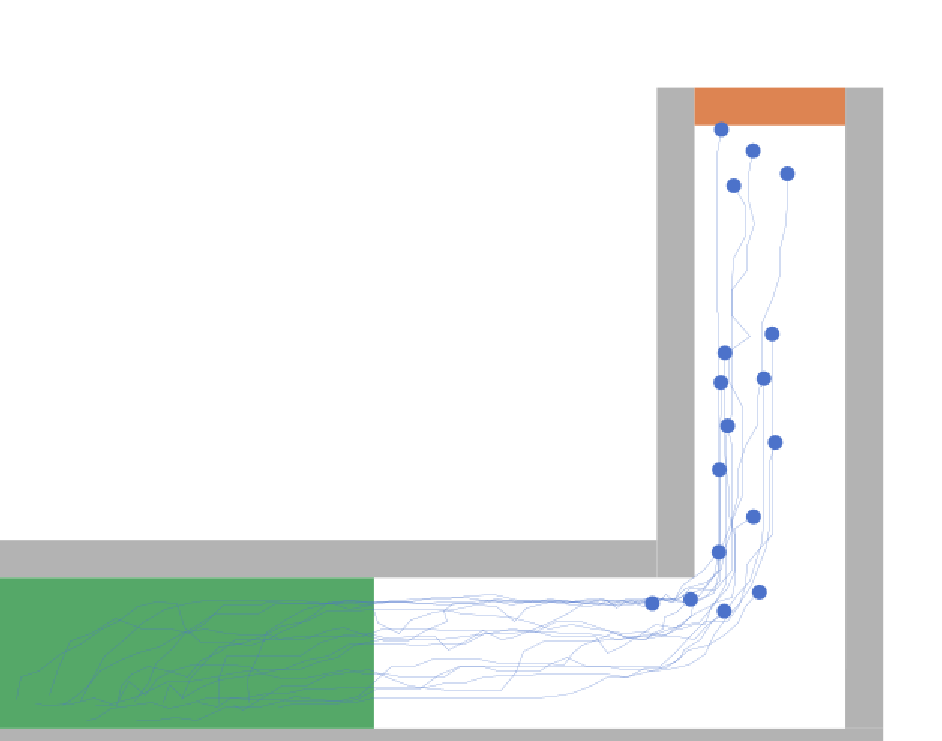
\includegraphics[scale=0.25]{report-template/images/rimea-6-run.png}}
\subfigure[ex1 RiMEA 6 end]{
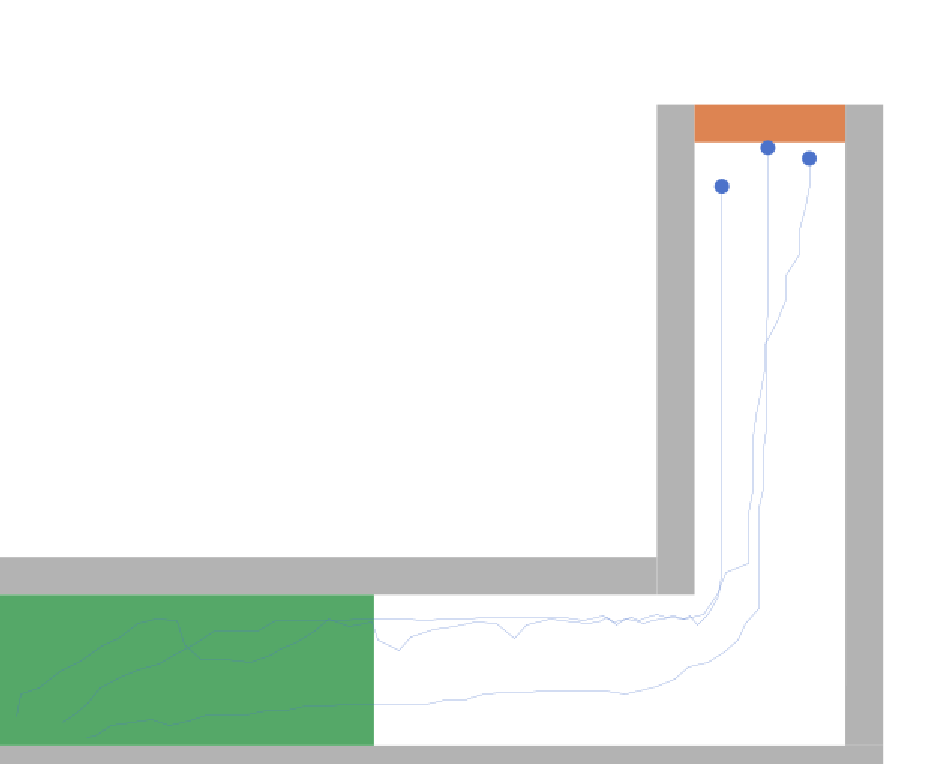
\includegraphics[scale=0.25]{report-template/images/rimea-6-fin.png}}
\subfigure[ex1 RiMEA 6 setup]{
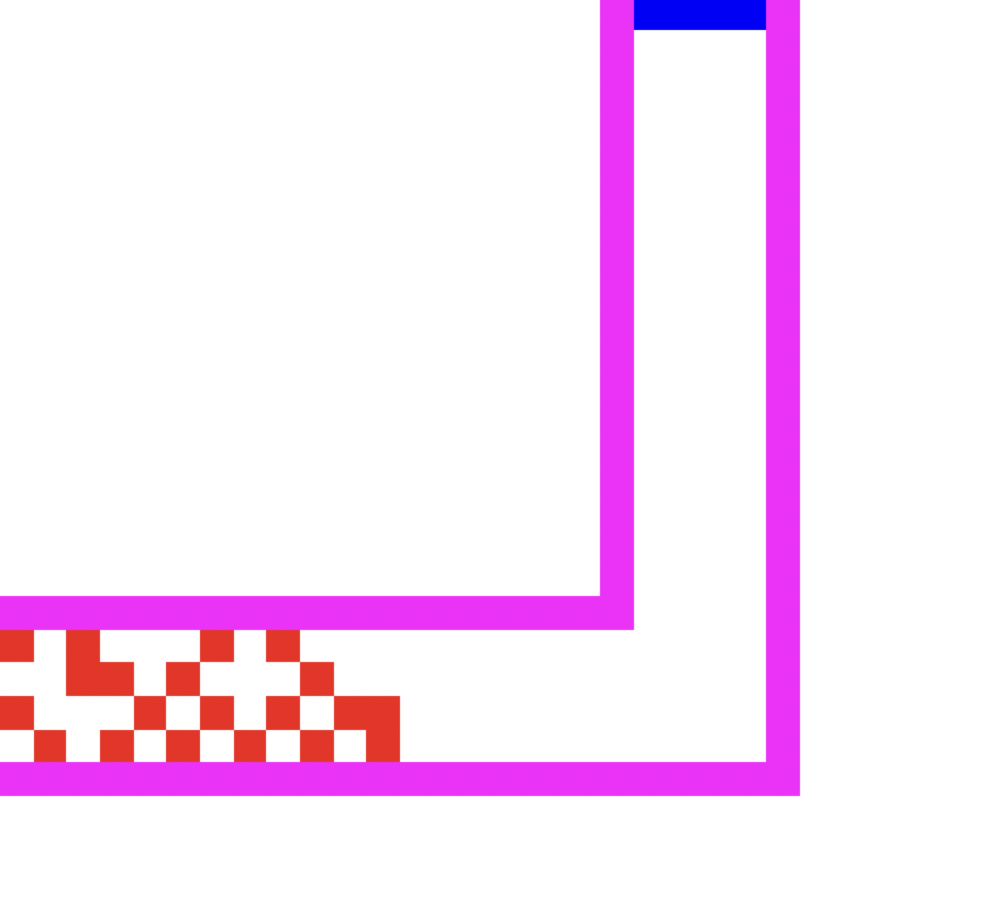
\includegraphics[scale=0.25]{report-template/images/old-rimea-6-setup.png}}
\subfigure[ex1 RiMEA 6 run]{
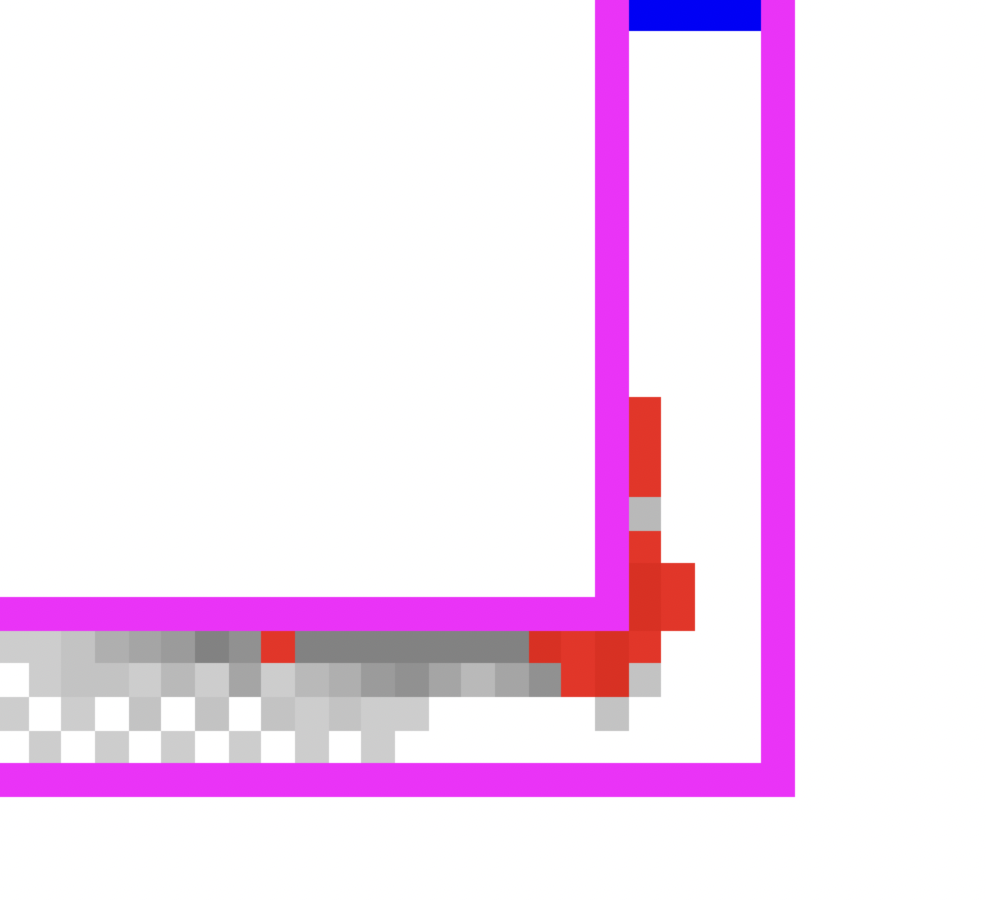
\includegraphics[scale=0.25]{report-template/images/old-rimea-6-run.png}}
\subfigure[ex1 RiMEA 6 finshed]{
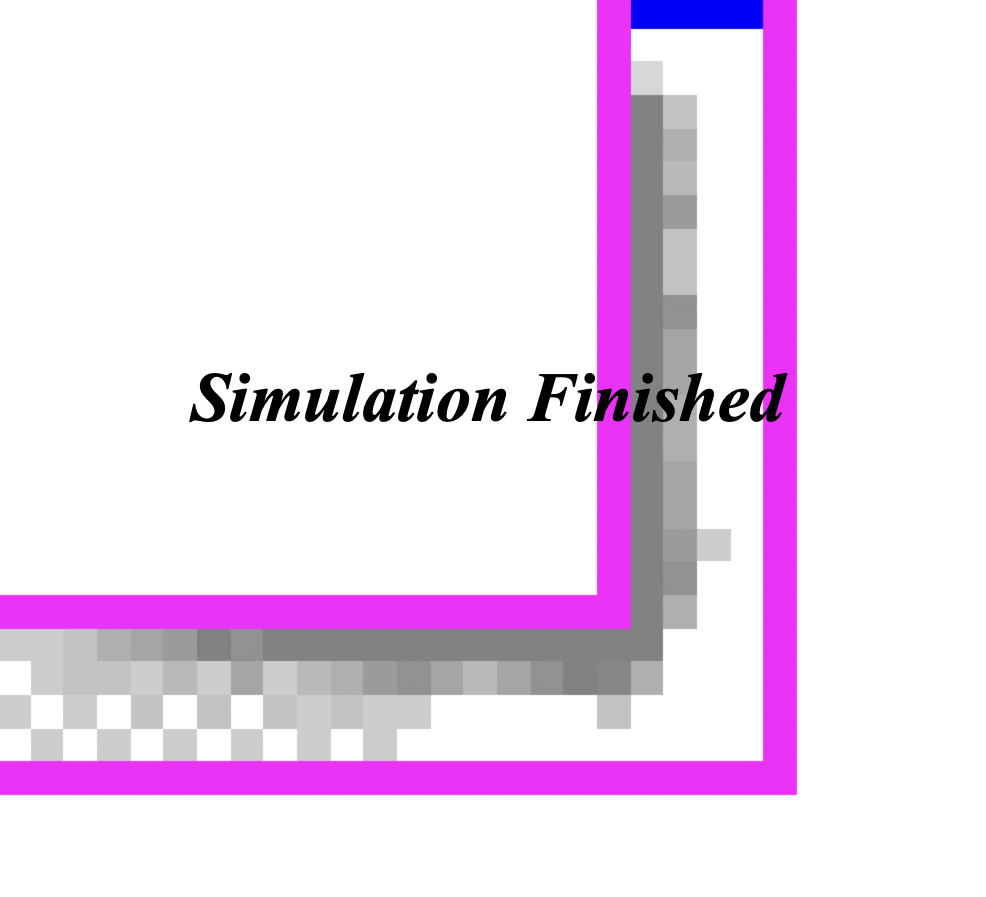
\includegraphics[scale=0.25]{report-template/images/old-rimea-6-fin.png}}
\caption{Comparison of RiMEA 6 simulations}
\label{rimea6}
\end{figure}


As shown in the Figure\ref{rimea6_setup}, the simulation setup utilized Vadere. The \texttt{Obstacle} tool was employed to create a corridor with a width of 4 units and a turning corner a 30x30 map. On the right side, the \texttt{Target} tool was used to establish a 4x1 rectangle, representing the exit. On the left side, the \texttt{Source} tool was employed to create a green area that generates 20 pedestrians. These pedestrians move at a speed of 0.5 \text{m/s}.

In Figure \ref{rimea6}, a comparison can be made between two simulations. In both experiments, pedestrians successfully navigate around the corner without passing through the walls. In the Vadere simulation using the Optimal Steps Model (OSM), pedestrians exhibit mutual repulsion, and not all of them cluster tightly while passing the corner. Instead, some pedestrians intentionally choose to walk on the outer side of the corner, maintaining a sufficient distance. However, in the simulation in exercise 1, pedestrians tend to take the shortest path, brushing the walls as they pass through the corner.

\paragraph{RiMEA Chicken test}

The purpose of the "Chicken Test" scenario is to assess obstacle avoidance. In the absence of obstacle avoidance, pedestrians would become trapped and unable to reach the target.

we used the \texttt{Obstacle} tool to create a fence with a width of 1 in a 50x50 map. Then, the \texttt{Target} tool was employed to establish a 1x1 exit directly below the obstacle. One Pedestrian are placed within the fenced area.

\begin{figure}[H] 
\centering
\subfigure[chicken test]{
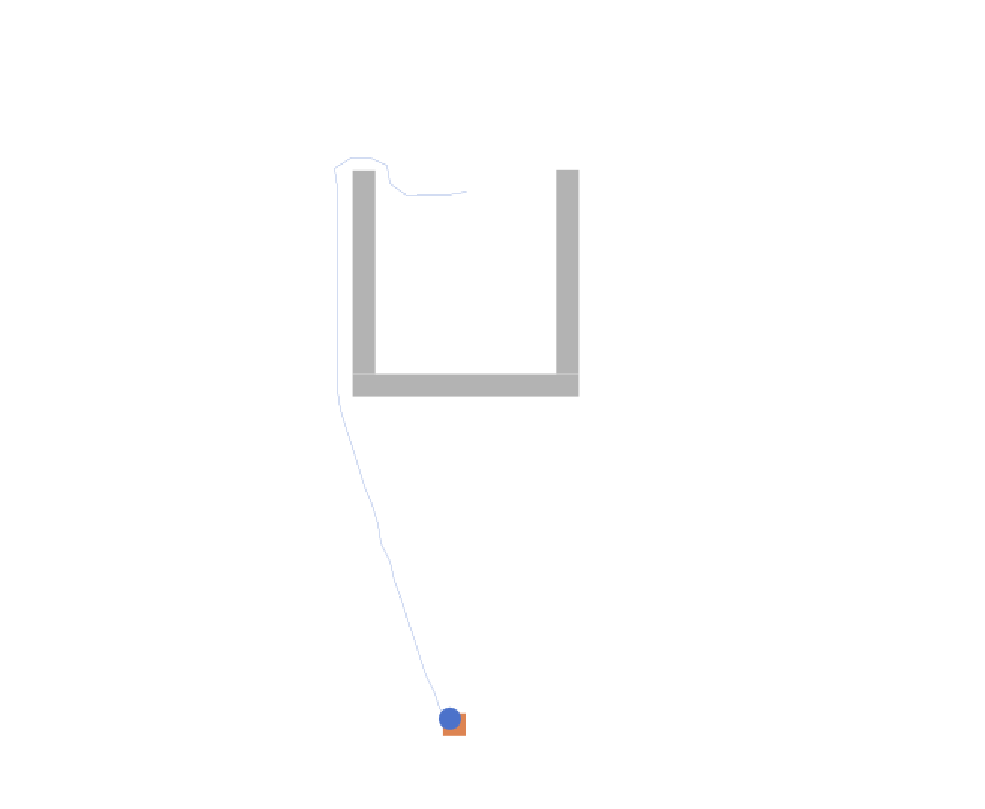
\includegraphics[scale=0.35]{report-template/images/chicken-test-clever.png}}
\subfigure[ex1 chicken test]{
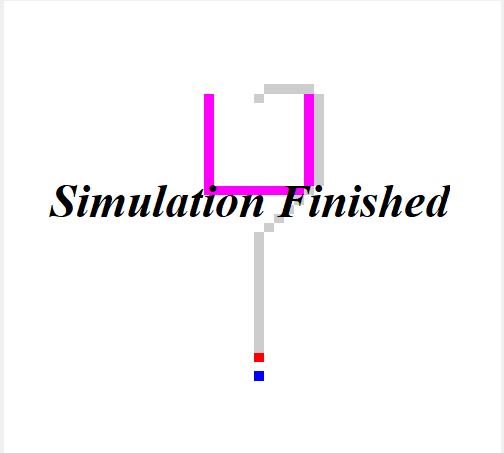
\includegraphics[scale=0.35]{report-template/images/old-chicken-test-clever.png}}
\caption{Comparison of chicken test}
\label{chicken-test}
\end{figure}

As shown in the Figure \ref{chicken-test}, although both simulations successfully navigate around the fence, their trajectories exhibit distinct differences. The most significant distinction is that, unlike in Exercise 1 where pedestrians tend to first move diagonally downward before transitioning to a straight downward movement, in the Vadere simulation, pedestrian, after circumventing the fence, proceed directly towards the exit.

\paragraph{Software Comparison}
In terms of visualization, Vadere uses different colors to represent elements. It offers an array of additional features for showcasing the movement process, including options to show/hide the walking direction of all pedestrians, show/hide the grid, and show/hide trajectories, etc. However, Vadere lacks the capability, present in our own cellular automaton from the first exercise, to retain the path lines of removed pedestrians on the map.
As far as the user interface is concerned, Vadere excels in scene creation compared to our own cellular automaton. It not only enables scene creation through mouse interaction but also allows users to input code for scene elements directly within the interface window.
\end{task}